\section{Livello Fisico}
    \subsection{Capacità massima di un canale}
        \problem
        Determinare la capacità massima del canale (bps) per un mezzo trasmissivo con larghezza di banda di 1 KHz e rapporto Segnale/Rumore = 1000.
        
        \solution
        Data la presenza di rumore si utilizza la formula:

        \begin{equation*}
            H \cdot log_2(1+S/N)
        \end{equation*}
        \begin{equation*}
            \centerline{$= 1KHz \cdot log_2(1001) = 10Kbps$}
        \end{equation*}

    \subsection{Determinazione ampiezza di banda}
        \problem
        Considerate un collegamento punto-punto in fibra ottica con lunghezza 100Km. Quale valore di ampiezza di banda (bit/s) rende un ritardo di propagazione uguale al tempo di trasmissione per pacchetti di 100byte?

        Disegnare il diagramma spazio tempo della comunicazione.

        \solution
        Calcolo il tempo di propagazione con $n$ (indice di rifrazione) nella fibra pari a 1.5:

        \begin{equation*}
            T_{pr} = l \cdot \frac{n}{c}
        \end{equation*}
        \begin{equation*}
            = 10^5m \cdot \frac{1.5}{2 \cdot 10^8  m/s} = 0.5 ~ ms
        \end{equation*}

        A partire dalla formula del tempo di trasmissione:

        \begin{equation*}
            T_{tr} = \frac{n}{Bitrate}
        \end{equation*}

        Calcolo l'ampiezza di banda:

        \begin{equation*}
            bitrate = \frac{800 ~ bit}{0.5 10^{-3} s}  = 1.6 ~ Mbit/s
        \end{equation*}

        \begin{center}
    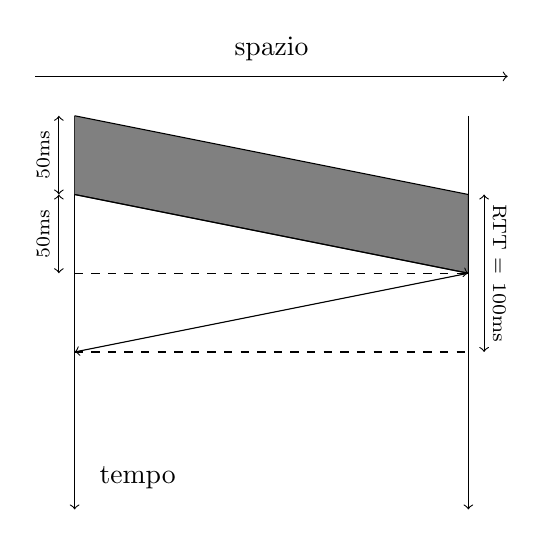
\begin{tikzpicture}
        % Vettore e testo per lo spazio
        \node[align=center] at (2.5,0.85) {spazio};
        \draw[->] (-0.5,0.5) -- (5.5,0.5);

        % Vettori e testo per il tempo
        \node at (0.8,-4.6) {tempo};
        \draw[->] (0,0) -- (0,-5);
        \draw[->] (5,0) -- (5,-5);

        % Scambio di messaggi
        \draw[fill=gray] (0,0) -- (5,-1) -- (5,-2) -- (0,-1);
        \draw[->] (0,-1) -- (5,-2);
        \draw[->] (5,-2) -- (0,-3);

        % Tratteggio di riferimento
        \draw[dashed] (0,-2) -- (5,-2);
        \draw[dashed] (0,-3) -- (5,-3);

        % Misurazioni
        \draw[<->] (-0.2, 0) -- (-0.2, -1);
        \node[rotate=90] at (-0.4,-0.5) {\scriptsize 50ms};
        \draw[<->] (-0.2, -1) -- (-0.2, -2);
        \node[rotate=90] at (-0.4,-1.5) {\scriptsize 50ms};
        \draw[<->] (5.2, -1) -- (5.2, -3);
        \node[rotate=270] at (5.4,-2) {\scriptsize RTT = 100ms};
    \end{tikzpicture}
\end{center}

    \subsection{Determinazione latenza}
        \problem
        Supporre una architettura di rete composta da un host A, host B e interconnessi dall'apparato di rete R.

        A comunica con R tramite etere a 10 Mbit/s per una distanza di 100 m.
        
        R comunica con B tramite fibra ottica a 1 Gbit/s per una distanza di 2000 m.
        
        L'apparato di rete può comportarsi nei seguenti modi:
        \begin{itemize}
            \item R memorizza il frame ricevuto da A; quando il frame è stato ricevuto completamente inizia subito la trasmissione verso B (store and forward)
            \item R introduce un tempo di inoltro $T_i(R) = 2 ms$ per ogni bit (cut through)
        \end{itemize}
        
        Realizzare il diagramma spazio tempo per i due casi e determinare il ritardo complessivo per un frame di 1 KB.

        \solution
        Calcolo i tempi di trasmissione e propagazione per ogni host e interconnessione, ricordando che $n$ vale:
        \begin{itemize}
            \item 1 per l'etere.
            \item 1.5 per la fibra ottica.
        \end{itemize}
        
        \begin{equation*}
            T_{tr}(A) = \frac{8K bit}{10Mb/s} = 800 \mu s
        \end{equation*}
        \begin{equation*}
            T_{pr}(\overline{AR}) = \frac{100m}{3 \cdot 10^8 m/s} = 0.33 \mu s
        \end{equation*}
        \begin{equation*}
            T_{tr}(R) = \frac{8Kbit}{1Gb/s} = 8 \mu s
        \end{equation*}
        \begin{equation*}
            T_{pr}(\overline{RB}) = 2000m \cdot \frac{1.5}{2 \cdot 10^8 m/s} = 10 \mu s
        \end{equation*}
        
        $Caso ~ 1: Ritardo = T_{tr}(A) + T_{pr}(\overline{AR}) + T_{tr}(R) + T_{pr}(\overline{RB}) = 818.33 \mu s$

        $Caso ~ 2: Ritardo = T_{tr}(A) + T_{pr}(\overline{AR}) + T_{tr}(R) + T_{pr}(\overline{RB}) + (n \cdot T_i(R)) = 16.82 ms$

        % Versione proposta dal professore che non avrebbe senso dato che il tempo di inoltro andrebbe applicato su ogni bit.
        %$Caso ~ 2: Ritardo =  T_{tr}(A) + TprAR + TiR + Tpr RB  = 812,33 \mu s$ \\

    \subsection{Determinazione dimensione canale}
        \problem
        Un canale trasmette alla velocità di 4 Kbps e ha un ritardo di propagazione di 20 ms. Si vuole usare l'algoritmo stop-and-wait con efficienza di almeno il 50\%, quali sono le dimensioni ammissibili dei frame?

        \solution
        L'efficienza del 50\% si ottiene avendo $T_{tr} \geq RTT$

        \begin{equation*}
            RTT = 2 T_{pr} = 40ms
        \end{equation*}
        \begin{equation*}
            n \geq 4 Kb/s \cdot 40 ms
        \end{equation*}
        \begin{equation*}
            n \geq 20 byte
        \end{equation*}